\subsubsection{Inner Product Space}

\paragraph{DistributionundefinedandundefinedTestundefinedFunctions}

\subparagraph{ContinousundefinedIndexing}

\subparagraph{DualityundefinedPairing}

\subparagraph{Exercises}

\begin{mystexercise}{$\delta$undefinedisundefinedaundefinedringundefinedhomomorphism}{delta_as_ring_homomorphism}\label{delta_as_ring_homomorphism}Considerundefined$\mathcal T$undefinedandundefined$\mathbb{R}$undefinedasundefinedtwoundefinedrings.

\textbf{1.undefinedProveundefinedthatundefined$\delta$undefinedpreservesundefinedringundefinedmultiplication}
\begin{equation}
f\delta(x)=f(0)\delta(x)
\end{equation}

\textbf{2.undefinedDistributionundefinedDerivativeundefinedofundefined$f\delta$}

Showundefinedthatundefinedtheundefineddistributionundefinedderivativeundefinedofundefined$f\delta$undefinedisundefined
\begin{equation}
\begin{aligned}
\delta[-fg'] &= f(0)\delta'[g]
\end{aligned}
\end{equation}
or,undefinedalternatively,
\begin{equation}
\delta[-fg']= \delta[f'g]+\delta'[fg]
\end{equation}

\end{mystexercise}
\begin{figure}[!htbp]
\centering
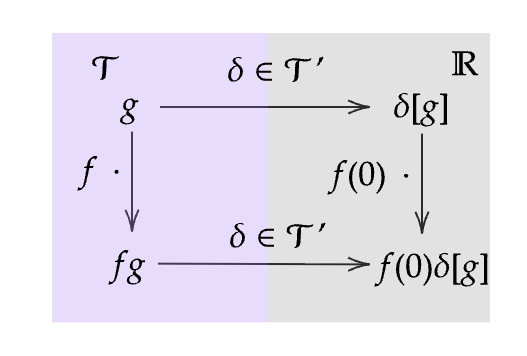
\includegraphics[width=0.7\linewidth]{files/T'_as_module-12b1670b351dbe8ed5bf4d60d4df5809.png}
\end{figure}

\begin{mystsolution}{SolutionundefinedtoundefinedExercise~\ref{delta_as_ring_homomorphism}}\begin{enumerate}
\item $\forall g\in \mathcal T$,undefinedweundefinedhave:

\begin{equation}
\begin{aligned}
(f\delta)[g] &= \delta[fg] \\
&=f(0)g(0) \\
&= f(0)\delta
\end{aligned}
\end{equation}


Asundefineddesired.


\item Weundefinedcanundefineddirecltyundefinedcomputeundefinedtheundefinedderivative:

\begin{equation}
\delta[f\phi] = f(0)\delta[\phi] \overset{\phi=-g'}{\Longrightarrow} \delta[f(-g')] = f(0)\delta[-g'] = f(0)\delta'(g)
\end{equation}


whereundefinedtheundefinedlastundefinedequalityundefinedusedundefinedtheundefineddefinitionundefinedofundefineddistributionundefinedderivative.
Nowundefinedweundefinedshowundefinedthatundefined$\delta[f'g]+\delta'[fg]=f(0)\delta'(g)$.undefinedWeundefineduseundefinedringundefinedhomomorphismundefinedpropertyundefinedtoundefinedestablish:

\begin{equation}
\begin{aligned}
\delta[f'g]+\delta'[fg] &= \delta[f']\delta[g]+\delta[-(fg')] \\
&= \delta[f']\delta[g]-(\delta[f']\delta[g]+\delta[f]\delta[g']) \\
&= -\underbrace{\delta[f]}_{f(0)}\delta[g'] \\
&= f(0)\delta'[g] \\
\end{aligned}
\end{equation}
\end{enumerate}

\end{mystsolution}
\begin{mystexercise}{$\delta^{(1/2)}$}{delta_1over2}\label{delta_1over2}Weundefinedcanundefineddefineundefinedtheundefineddistributionundefined$\delta^{(1/2)}$undefinedundefinedasundefinedaundefinedfourierundefinedtransformundefinedofundefined$|k|^{1/2}$:
\begin{equation}
\delta^{(1/2)}=\frac{1}{2\pi}\int_{-\infty}^{\infty} |k|^{1/2}\exp(ikx)dk
\end{equation}

Theundefinedfourierundefinedtransformundefinedisundefinedclearlyundefineddivergent,undefinedhenceundefinedweundefinedcanundefinedaddundefinedaundefinedregulator.undefinedDefine:
\begin{equation}
\begin{aligned}
\delta^{(1/2)}_{\mu}&=\frac{1}{2\pi}\int_{-\infty}^{\infty} |k|^{1/2}\exp(ikx)\exp(-\mu|k|)dk \\
&= \frac{1}{2\pi}\int_{-\infty}^{\infty} |k|^{1/2}\exp(ikx-\mu|k|)dk
\end{aligned}
\end{equation}

\begin{enumerate}
\item Evaluateundefinedtheundefinedintegralundefinedgetundefinedaundefinedclosedundefinedformundefinedexpressionundefinedofundefined$\delta_{\mu}^{(1/2)}$undefinedby:

\begin{itemize}
\item Splittingundefined$k<0$undefinedandundefined$k>0$
\item Changeundefinedvariableundefinedtoundefined$y=|k|^{1/2}$
\item Writeundefinedtheundefinedresultundefinedasundefined$\frac{d}{d\mu}$undefinedofundefinedaundefinedGaussianundefinedintegral
\item Useundefinedtheundefinedtrignometricundefinedrelation

\begin{equation}
\arctan(z)=\frac{i}{2}\log\left(\frac{1-iz}{1+iz}\right)
\end{equation}
\end{itemize}


\item Investigateundefined$\delta^{(1/2)}_{\mu}$undefinedby:

\begin{itemize}
\item Sketchundefined$\delta^{(1/2)}_{\mu}$undefinedforundefineddifferentundefined$\mu$
\item Computeundefinedtheundefinedzerosundefinedofundefined$\delta^{(1/2)}_{\mu}$
\end{itemize}


\item Showundefinedthatundefined$\delta^{(1/2)}_{\mu}$undefinedisundefinedtheundefinedfourierundefinedtransformundefinedofundefinedaundefinedfunctionundefinedthatundefinedvanishesundefinedatundefined$k=0$.undefinedWhatundefinedpropertyundefinedofundefined$\delta^{(1/2)}_{\mu}$undefinedcanundefinedweundefinedinfer?
\item Computeundefinedtheundefinedlimit
$\lim_{\mu \to 0^+}\delta^{(1/2)}_{\mu}$
\item Assumingundefinedthatundefinedforundefined$|x|>\max|\{x_0: \delta^{(1/2)}_{\mu}(x_0)=0\}|$,undefinedtheundefinedconvergenceundefinedof

\begin{equation}
\delta^{(1/2)}_{\mu} \rightarrow \delta^{(1/2)}
\end{equation}


isundefinedpointwise.undefinedDeduce:

\begin{equation}
\int_{-\infty}^{\infty}\delta^{(1/2)}=-\sqrt{\frac{1}{8\pi}} \int_{-\infty}^{\infty} \frac{1}{|x|^{3/2}}\{\phi(x)-\phi(0)\}dx
\end{equation}
\end{enumerate}

\end{mystexercise}
\begin{mystsolution}{SolutionundefinedtoundefinedExercise~\ref{delta_1over2}}\begin{enumerate}
\item Followingundefinedtheundefinedguide:

\begin{equation}
\begin{aligned}
\delta^{(1/2)}_{\mu} &= \frac{1}{2\pi}\left\{\int_{-\infty}^0 (-k)^{1/2} \exp(ikx+\mu k)dk + \int_{0}^{\infty} (k)^{1/2} \exp(ikx-\mu k)dk 
\right\} \\
&= 
\frac{1}{2\pi}\left\{\underbrace{\int_{-\infty}^0 y \exp(-iy^2x-\mu y^2)dk}_{A} + \underbrace{\int_{0}^{\infty} y\exp(iy^2x-\mu y^2)dk}_{B} 
\right\} \\
\end{aligned}
\end{equation}
\end{enumerate}

\end{mystsolution}
\paragraph{Formalundefinedadjoint}

\paragraph{ConcreteundefinedAdjoint}

\subparagraph{TheundefinedSturm-LiouvilleundefinedOperator}

Theundefined\textbf{Sturm-Liouvilleundefinedoperator}undefinedisundefinedaundefinedlinearundefineddifferentialundefinedoperatorundefinedofundefinedtheundefinedform
\begin{equation}
\mathcal L=-\frac{d}{dx}\left(p\frac{d}{dx}y\right)+q\frac{d}{dx}
\end{equation}

We'veundefinedshownundefinedthatundefinedtheundefinedSturm-Liouvilleundefinedopeartorundefinedisundefinedself-adjointundefinedwithundefinedappropriateundefinedboundaryundefinedconditionundefinedinundefinedtheundefinedsenseundefinedthat:
\begin{equation}
\begin{aligned}
\langle u, \mathcal Lv \rangle &= \langle \mathcal L^*u, v \rangle
\end{aligned}
\end{equation}
henceundefineditundefinedisundefinedanalgousundefinedtoundefinedself-adjointundefinedoperatorundefinedinundefinedfinite-dimensionalundefinedvectorundefinedspaces,undefinedwhichundefinedasundefinedsymmetricundefinedmatrixundefinedrepresentationundefinedwhenundefinedtheundefinedunderlyingundefinedfieldundefinedisundefinedreal.undefinedWeundefinednowundefinedmakeundefinedthisundefinedconnectionundefinedexplicit,undefinedi.e.,undefinedactuallyundefinedconstructingundefinedtheundefineddiscretized,undefinedfinite-dimensionalundefinedmatrixundefinedrepresentationundefinedofundefinedtheundefinedSturm-LiouvilleundefinedOperator.

\subparagraph{AundefinedDiscreteundefinedAnalog}

Let'sundefinedconsiderundefinedaundefinedconcreteundefinedSLundefinedopeartorundefineddefinedundefinedonundefined$[0,1]$undefinedwithundefinedDirchletundefinedboundaryundefinedconditionundefined$y(0)=y(1)=0$.undefinedInsteadundefinedofundefineddirectlyundefineddiscretizingundefined$\mathcal L$,undefinedweundefinedaimundefinedtoundefinedfindundefinedaundefinedmatrixundefined$L$undefinedsuchundefinedthatundefineddiscretizesundefinedtheundefinedquadraticundefinedform:
\begin{equation}
F(y)=\int y\mathcal Ly dx \rightarrow \hat y^TL\hat y
\end{equation}
Firstundefinedweundefinednoteundefinedthat:
\begin{equation}
\label{func}
\begin{aligned}
F(y) &= \int_0^1 y\left(-\frac{d}{dx}\left(p\frac{d}{dx}y\right) + qy\right) dx \\
&= \int_0^1 -y \frac{d}{dx}\left(p\frac{d}{dx}y\right)dx+\int_0^1 qy^2dx  \\
&= -\left\{\cancel{\left[yp\frac{dy}{dx}\right]_0^1} - \int p\left(\frac{dy}{dx}\right)^2 \right\} + \int_0^1 qy^2dx \\
&= \int_0^1 py'^2 + qy^2
\end{aligned}
\end{equation}
Nowundefinedweundefineddiscretizeundefined$y, p, q$undefinedtoundefined$N$-dimensionalundefinedarrays:
\begin{equation}
\begin{aligned}
\hat y &= [y_1,...,y_N] \\
\hat p &= [p_1,...,p_N] \\
\hat q &= [q_1,...,q_N]
\end{aligned}
\end{equation}
Usingundefinedforwardundefineddifferenceundefinedweundefinedget:
\begin{equation}
\hat y =\left(\frac{y_{i+1}-y_i}{h}\right)^2
\end{equation}
Rewriteundefinedtheundefinedintegralundefinedasundefinedaundefinedfiniteundefinedsumundefinedweundefinedobtainundefinedaundefineddiscretizedundefinedversionundefinedofundefined(\ref{func}):
\begin{equation}
\boxed{\hat F(\hat y)=\sum_{i=1}^N h p_i\left(\frac{y_{i+1}-y_i}{h}\right)^2 +q_iy_i^2}
\end{equation}
Ourundefinedgoalundefinedisundefinednowundefinedtoundefinedfindundefinedaundefinedmatrixundefined$L$undefinedsuchundefinedthatundefined$\hat y^TL\hat y=\hat F(\hat y)$.undefinedRewriteundefined$\hat F(\hat y)$:
\begin{equation}
\hat F(\hat y) =\sum_{i=1}^N Np_i(y_{i+1}^2 -2y_{i+1}y_i +y_i^2)+\frac{1}{N}q_iy_i^2
\end{equation}
Weundefinedcanundefinedsplitundefined$L=L_1+L_2$undefinedsuchundefinedthat

\begin{enumerate}
\item $\hat y^T L_1 \hat y = \sum_{i=1}^N Np_i(y_{i+1}^2 -2y_{i+1}y_i +y_i^2)$
\item $\hat y^T L_2 \hat y = \sum_{i=1}^N \frac{1}{N}q_iy_i^2$.
\end{enumerate}

\textbf{(Constructingundefined$L_1$)}
Let'sundefinedfirstundefineddealundefinedwithundefined$L_1$.undefinedConsiderundefinedtheundefined$2\times 2$blockundefinedwithundefinedtheundefinedupperleftundefinedcornerundefinedatundefined$(i,i)$undefinedthatundefinedshould
representundefined$Np_i(y_{i+1}^2 -2y_{i+1}y_i +y_i^2)$.undefinedThisundefinedisundefinedeasy:
\begin{equation}
\begin{aligned}
A_i=Np_i\begin{pmatrix}
1 & -1\\
-1 & 1 \\
\end{pmatrix}
\end{aligned}
\end{equation}
Toundefinedassembleundefined$L_1$undefinedweundefinedcanundefinedoverlapundefined$A_i$undefinedalongundefinedtheundefineddiagonalundefinedofundefined$L$undefinedwithundefinedaundefinedstrideundefinedofundefined1.undefinedConcretely:

\begin{mystcodebox}
\begin{verbatim}
for i=1,...,N -1
    L[i,i] += Np_i
    L[i+1,i+1] += Np_i
    L[i,i+1] -= Np_i 
    L[i+1,i] -= Np_i
\end{verbatim}

\end{mystcodebox}
\begin{mystthmexample}{}{example-innerproductspace-1}Aundefinedquickundefinedexampleundefinedforundefined$N=4$:
\begin{equation}
\begin{aligned}
4\begin{pmatrix}
p_1 & -p_1 & 0 & 0 \\
-p_1 & p_1+p_2 & -p_2 &0 \\
0 & -p_2 & p_2+p_3 & -p_3 \\
0 &  0 & -p_3  & p_3
\end{pmatrix}
\end{aligned}
\end{equation}

\end{mystthmexample}
\textbf{(Constructingundefined$L_2$)}
$L_2$undefinedisundefinedpurelyundefineddiagonalundefinedandundefinedisundefinedeasierundefinedtoundefinedderive.undefinedSinceundefineditundefinedonlyundefinedhasundefinedquadraticundefinedtermundefined$y_i^2$,undefinedatundefinedeachundefinedrowundefined$i$undefinedweundefinedonlyundefinedneedundefinedtoundefinedincludeundefined$y_i$.undefinedHence:
\begin{equation}
\begin{aligned}
L_2 = \frac{1}{N}\begin{pmatrix}q_1 & & \\
& \ddots & \\
& & q_N
\end{pmatrix}
\end{aligned}
\end{equation}

\textbf{(Assemblyundefined$L_1+L_2$)}
Itundefinedisundefinedclearundefinedthatundefined$L$undefinedshouldundefinedlookundefinedlike:

\begin{equation}
\begin{aligned}
L=N\begin{pmatrix}
p_1&  -p_1 & & &  \\
-p_1& p_1+p_2 &  -p_2 & &  \\
&  \ddots  &  \ddots &   \ddots &   \\
&  &-p_{N-1} &p_{N-1}+p_{N} & -p_N  \\
& & &-p_N & p_N \\
\end{pmatrix} 
+ 
\frac{1}{N}\begin{pmatrix}q_1 & & \\
& \ddots & \\
& & q_N
\end{pmatrix}
\end{aligned}
\end{equation}

However,undefinedsinceundefinedweundefinedareundefineddealingundefinedwithundefinedconcreteundefinedoperatorsundefinedwithundefinedaccompanyingundefineddomainundefinedandundefinedboundaryundefinedcondition,undefinedweundefinedneedundefinedtoundefinedencoorperateundefinedtheundefinedDircheltundefinedboundaryundefinedconditionundefined$y(0)=1, y(1)=0$undefinedintoundefined$L$.undefinedToundefineddoundefinedsoundefinedweundefinedneedundefinedtoundefinedzero-outundefinedtheundefinedfirstundefinedrowundefinedandundefinedcolumnundefinedofundefined$L$.undefinedHenceundefinedfinallyundefinedweundefinedget:

\begin{mystthmproposition}{}{proposition-innerproductspace-2}TheundefinedSturm-LiouvilleundefinedOperatorundefinedonundefined$[0,1]$undefinedwithundefinedDirchletundefinedboundaryundefinedconditionundefined$y(0)=y(1)$undefinedcanundefinedbeundefineddiscretizedundefinedas
\begin{equation}
\label{discreteSL}
\begin{aligned}
L=N\begin{pmatrix}
0 &0 & & &  &\\
0 &p_1+p_2 & -p_2& & & \\
&-p_2&  \ddots &\ddots & -p_{N-1}& \\
& & \ddots &-p_{N-1} & p_{N-1}+p_N &0 \\
& & & &0 & 0\\
\end{pmatrix} 
+ 
\frac{1}{N}\begin{pmatrix}0 & & & & \\
& q_2 & & & \\
&  & \ddots& & \\
& & & q_{N-1} & \\
& &  & & 0  \\
\end{pmatrix}
\end{aligned}
\end{equation}

\end{mystthmproposition}
Weundefinedcanundefinedseeundefinedthatundefined$L$undefinedisundefinedindeedundefinedaundefinedsymmetricundefinedrealundefinedmatrix(Hermitian)!

\textbf{NumpyundefinedImplementation}
Thisundefinedcanundefinedeasilyundefinedbeundefinedtranslatedundefinedtoundefinednaiveundefined\texttt{numpy}undefinedcode:

\begin{mystcodebox}
\begin{verbatim}
class SturmLiouville:
    def __init__(self,N, p, q=None, grid='forward'):
        A = np.zeros(shape=(N,N))
        if grid == 'forward':
            for i in range(N -1):
                A[i, i] += p[i]
                A[i+1, i+1] += p[i]
                A[i, i+1] -= p[i]
                A[i+1, i] -= p[i]

        if q is not None:
            I = np.eye(N) 
            L = A + q @ I
        else:
            L = A
        
        # Dirchlet Boundary Condition
            L[0,0]=0.0
            L[0,1]=0.0
            L[1,0]=0.0
            L[N -1,N -1]=0.0
            L[N -1,N -2]=0.0
            L[N -2,N -1]=0.0
        self.L = (L * N ** 2)
        self.N = N

    def solve_eigen(self, top_k=10):
        eval, evec = np.linalg.eig(self.L)
        top_k_idx = np.argsort(eval[eval>0])[:top_k]
        return eval[top_k_idx] , evec[:, top_k_idx], top_k_idx
\end{verbatim}

\end{mystcodebox}
\textbf{Example:undefined$-\frac{d^2}{dx^2}$undefinedasundefinedaundefinedMatrix}
Weundefinedcanundefineddoundefinedaundefinedquickundefinedexampleundefinedtoundefinedshowcaseundefinedthatundefined$L$undefinedisundefinedindeedundefinedaundefineddiscretizationundefinedofundefined$\mathcal L$.

\begin{mystthmexample}{-$\frac{d^2}{dx^2}$}{example-innerproductspace-3}Weundefinedhaveundefinedalreadyundefinedseenundefinedthatundefinedtheundefinedopeartor:
\begin{equation}
T=-\frac{d^2}{dx^2}, D(T)=\{y,Ty \in L^2[0,1]:y(0)=y(1)=0\}
\end{equation}
hasundefinedeigenvaluesundefinedandundefinedeigenvectors:
\begin{equation}
\begin{aligned}
y_j(x) &=\sqrt{2}\sin j\pi x \\
\lambda_j &= j^2\pi^2
\end{aligned}
\end{equation}
forundefined$j=1,2,3...$.undefinedTheundefinedproblemundefinedisundefinedthat,undefinedcanundefinedweundefinedsolveundefinedaundefinedmatrixundefinedeigenvalueundefinedproblemundefinedtoundefinedrecoverundefinedexactlyundefinedtheundefinedsameundefinedresult?
Indeedundefinedweundefinedcan!undefinedPassingundefined$p= -1$undefinedandundefined$q=0$undefinedgetsundefinedus:
\begin{equation}
\begin{aligned}
L=N\begin{pmatrix}
0 & 0 & &  &  \\
0 & 2 & -1 & &  \\
 & -1 & \ddots & \ddots & \\
& & \ddots & 2 & -1  &\\
& & & -1& 2 & 0\\
& & & & 0 & 0 \\
\end{pmatrix}
\end{aligned}
\end{equation}

andundefinedsolvingundefinedtheundefinedmatrixundefinedeigenvalueundefinedproblemundefined
\begin{equation}
\begin{aligned}
L\hat y &= \lambda \hat y
\end{aligned}
\end{equation}
undefinedgetsundefinedus:
\footnote{Sinceundefinediterativeundefinedeigensolversundefinedgivesundefinedeigenvectorsundefinedofundefinedarbitraryundefinedmagnitudeundefined$v_j=a\sin(j\pi(x))$,undefinedweundefinedneedundefinedtoundefinednormalizeundefinedproperlyundefinedby
1.Ensureundefined$a>0$

\begin{enumerate}
\item Divideundefinedbyundefined$\sqrt{\sum y_i^2 h}$
\end{enumerate}}

\end{mystthmexample}
\begin{figure}[!htbp]
\centering
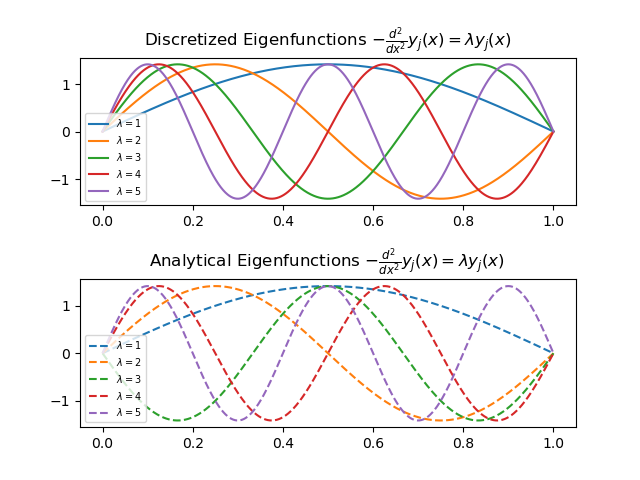
\includegraphics[width=0.7\linewidth]{files/sl_evecs-749bd46b634f4b726002411b1a849030.png}
\end{figure}

\begin{mystexercise}{}{exercise-uyplae01a4}\label{exercise-uYPlAE01a4}\label{exercise-uyplae01a4}\begin{enumerate}
\item Weundefineddiscretizedundefined$L$undefinedbasedundefinedonundefinedtheundefinedquadraticundefinedformundefined$\int_0^1 y\mathcal L y dx$,undefinedhenceundefined$\hat y^T L\hat y$undefinedshouldundefinedcoincideundefinedwithundefined$\int_0^1 y\mathcal L y dx$.undefinedComeundefinedupundefinedwithundefinedatundefinedleastundefined2undefinedfunctionsundefinedandundefined2undefinedoperatorsundefinedthatundefinedsatisfyundefinedtheundefinedrequirment($L^2(0,1),y(0)=y(1)=0$).undefinedComputeundefinedtheundefinedquadraticundefinedformundefinedanalyticallyundefinedandundefinednumericaly.undefinedCheeckundefinedthatundefinedtheundefinedresultsundefinedareundefinedtheundefinedsame.
\item Removeundefinedtheundefinedmaskingundefinedcodeundefinedsnippet(whichundefinedimplementsundefinedDirchletundefinedboundaryundefinedcondition)undefinedinundefinedtheundefinednaiveundefinedSLundefinedclassundefined\texttt{SturmLiouville}.undefinedWhatundefinedisundefinedtheundefinedresultingundefinedeigenvectors?undefinedExplainundefinedtheundefinedresult.
\item Tryundefinedcomingundefinedupundefinedwithundefineddifferentundefineddiscretizationundefinedwithundefinedcenterundefineddifferenceundefinedorundefinedbackundefineddifference.undefinedImplemetundefineditundefinedinundefined\texttt{python}
orundefined\texttt{julia}.

\begin{itemize}
\item Isundefinedtheundefinedresultingundefinedmatrixundefined$L$undefinedstillundefinedsymmetricundefined?
\item Centerundefineddifferencingundefinedschemeundefinedresultsundefinedinundefinedaundefinednumericalundefinedartifcat,undefinedwhatundefinedisundefinedtheundefinednumericalundefinedartifact?undefinedTryundefinedexplainingundefinedwhyundefinedsuchundefinedartifactundefinedoccur(\textit{Hint:undefinedNoteundefinedthatundefinedevenundefinedandundefinedodddundefinedindiciesundefinedareundefineddecoupled})
\end{itemize}
\end{enumerate}

\end{mystexercise}
%  
% :::{note} Optimizing $x^TAx$ gives $Ax=\lambda x$
% Let $x\in \mathbb{R}^n$, $A\in \mathbb{R^{n\times n}}$ is a **symmetric** matrix, define:
% $$
% F(x)=\frac12 \langle x,Ax \rangle
% $$
% Consider the optimization of $F$ constrained on $\|x\|^2=1$ 
% :::
% 
% We use lagarange multiplier:
% $$
% (Ax)^T+x^TA-2\lambda x^T &=0 \\
% Ax + A^Tx - 2\lambda x &=0 \\
% 2(A-\lambda I)x&=0 \\
% Ax &= \lambda x
% $$ 
% [^diff]
% Subjected to $\|x\|^2=1$. We note that this is an **eigenvalue problem**. 
%